%----------------------------------------------------------------------------------------
%	PACKAGES AND OTHER DOCUMENT CONFIGURATIONS
%------------------------------------------------------------------------
\documentclass[11pt]{article}
\usepackage[utf8]{inputenc} % Required for inputting international characters
\usepackage[T1]{fontenc} % Output font encoding for international characters
\usepackage{mathpazo} % Palatino font
\usepackage[czech]{babel} % Czech
\usepackage{graphicx}  % Graphics
\usepackage{caption}  % Caption
%\usepackage[amsmath]
\usepackage{placeins}

\begin{document}

%----------------------------------------------------------------------------------------
%	TITLE PAGE
%----------------------------------------------------------------------------------------

\begin{titlepage} % Suppresses displaying the page number on the title page and the subsequent page counts as page 1
	\newcommand{\HRule}{\rule{\linewidth}{0.5mm}} % Defines a new command for horizontal lines, change thickness here
	
	\center % Centre everything on the page
	
	%------------------------------------------------
	%	Headings
	%------------------------------------------------
	
	\textsc{\LARGE České vysoké učení technické v Praze}\\[1.5cm] % Main heading such as the name of your university/college
	
	\textsc{\Large Algoritmy digitální kartografie a GIS}\\[0.5cm] % Major heading such as course name
	
	\textsc{\large Katedra geomatiky}\\[0.5cm] % Minor heading such as course title
	
	%------------------------------------------------
	%	Title
	%------------------------------------------------
	
	\HRule\\[0.4cm]
	
	{\huge\bfseries Úloha č. 4: Množinové operace s polygony}\\[0.4cm] % Title of your document
	
	\HRule\\[1.5cm]
	
	%------------------------------------------------
	%	Author(s)
	%------------------------------------------------
	
	

	
	% If you don't want a supervisor, uncomment the two lines below and comment the code above
	Monika \textsc{Křížová} % Your name
	
	Marek \textsc{Hoffmann}
	
	%------------------------------------------------
	%	Date
	%------------------------------------------------
	
	\vfill\vfill\vfill % Position the date 3/4 down the remaining page
	
	{\large leden 2022} % Date, change the \today to a set date if you want to be precise
	
	%------------------------------------------------
	%	Logo
	%------------------------------------------------
	
	%\vfill\vfill
	%\includegraphics[width=0.2\textwidth]{placeholder.jpg}\\[1cm] % Include a department/university logo - this will require the graphicx package
	 
	%----------------------------------------------------------------------------------------
	
	\vfill % Push the date up 1/4 of the remaining page
	
\end{titlepage}

%----------------------------------------------------------------------------------------


%----------------------------------------------------------------------------------------
%	TABLE OF CONTENT
%----------------------------------------------------------------------------------------

\tableofcontents
%\thispagestyle{empty}

\clearpage

%----------------------------------------------------------------------------------------
%	ZADÁNÍ
%----------------------------------------------------------------------------------------

\section{Zadání}

%----------------------------------------------------------------------------------------
%	BONUSOVÉ ÚLOHY
%----------------------------------------------------------------------------------------

\section{Údaje o bonusových úlohách}

\begin{itemize}
	\item 
	\item 
	\item 	
\end{itemize}

%----------------------------------------------------------------------------------------
%	POPIS PROBLÉMU
%----------------------------------------------------------------------------------------

\section{Popis problému}

 
%----------------------------------------------------------------------------------------
%	POPIS ALGORITMŮ
%----------------------------------------------------------------------------------------

\section{Popisy algoritmů}

%----------------------------------------------------------------------------------------
%	PROBLEMATICKÉ SITUACE
%----------------------------------------------------------------------------------------
\section{Problematické situace}
	


%----------------------------------------------------------------------------------------
%	VSTUPNÍ DATA
%----------------------------------------------------------------------------------------


\section{Vstupní data}
\subsection{Načítání textového souboru}

Soubor polygonů určenými body s polohovými souřadnicemi x, y v souřadnicovém systému S-JTSK se do projektu nahrávají po stisknutí  tlačítka \textit{Load polygons}.

Body jsou načítány postupně řádek po řádku, přičemž musí v nahrávaném souboru platit následující pravidla:    

\begin{itemize}
\item na řádku je pořadí proměnných id >> y (S-JTSK) >> x (S-JTSK),  hodnoty jsou od sebe odděleny jednou mezerou,
\item id je identifikátor jednotlivých vrcholů polygonu, x, y, jsou polohové souřadnice vrcholu polygonu

\end{itemize}

\begin{figure}[htbh]
	\centering	
	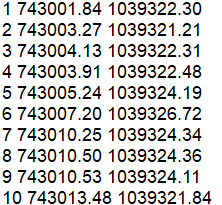
\includegraphics[scale=1]{images/vstup_polygon.png} 
	\caption{Špagetový model vstupního souboru bodů}
	\label{fig:vstup.}
\end{figure} 
\FloatBarrier

\begin{figure}[htbh]
	\centering
	\captionsetup{justification=centering}
	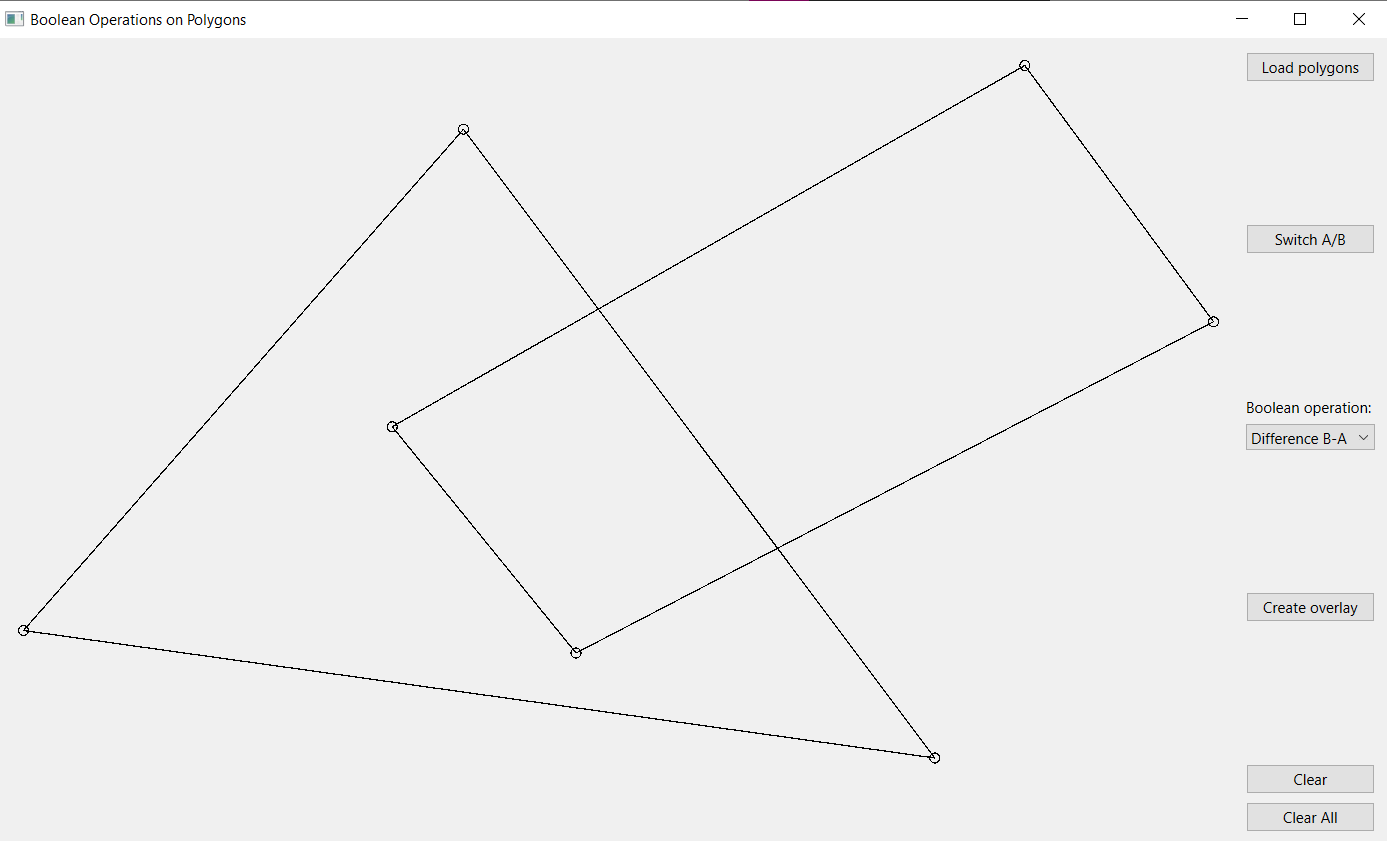
\includegraphics[scale=0.42]{images/vystup_LoadPoints.png} 
	\caption{Aplikace po načtení polygonů z textového souboru}
	\label{fig:vystup_LoadPoints}	
\end{figure} 
\FloatBarrier

\subsection{Kreslení polygonů}
Druhou možností zadávání polygonů je kreslení polygonů přímo v interaktivním prostředí aplikace. Opakovaným zadáváním bodů kliknutím myši lze vytvořit polygon jakéhokoliv tvaru. Po stisknutí tlačítka \textit{Switch A/B} lze stejným způsobem zadat druhý polygon. Nad touto dvojící pak lze provádět vybrané množinové operace.

\begin{figure}[htbh]
	\centering
	\captionsetup{justification=centering}
	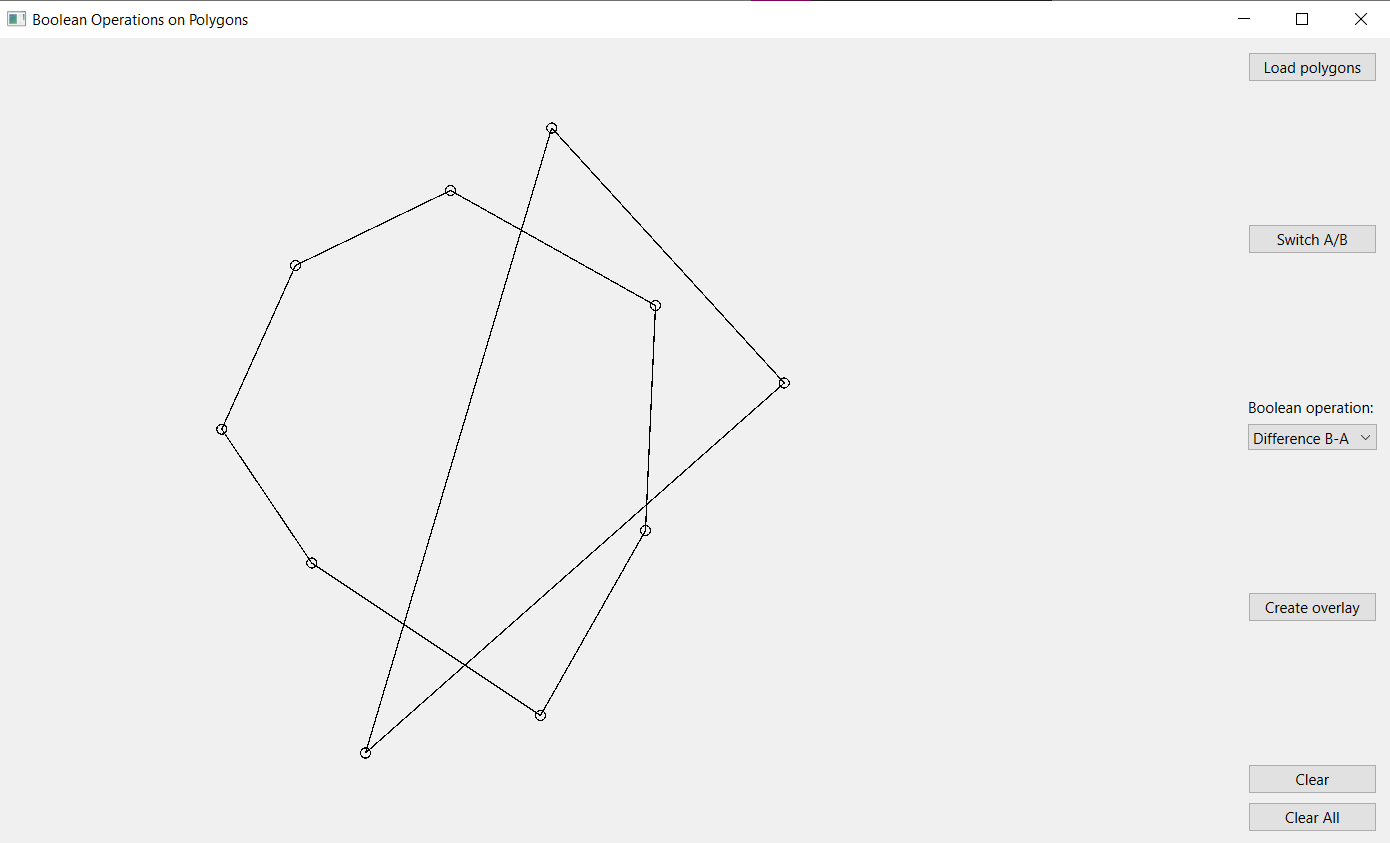
\includegraphics[scale=0.42]{images/vstup_kresleni.png} 
	\caption{Aplikace po manuálním nakreslení dvou polygonů}
	\label{fig:vstup_kresleni}	
\end{figure} 
\FloatBarrier

%----------------------------------------------------------------------------------------
%	VÝSTUPNÍ DATA
%----------------------------------------------------------------------------------------
\section{Výstupní data}

Nad zadanými polygony lze na základě výběru z comboBoxu provést 4 základní množinové operace; sjednocení (\ref{fig:vystup_union}), průnik (\ref{fig:vystup_intersection}) a rozdíl polygonů A-B a B-A (\ref{fig:vystup_diffAB}, \ref{fig:vystup_diffBA}). Jednotlivé operace jsou zobrazeny na následujících obrázcích.

\begin{figure}[htbh]
	\centering
	\captionsetup{justification=centering}
	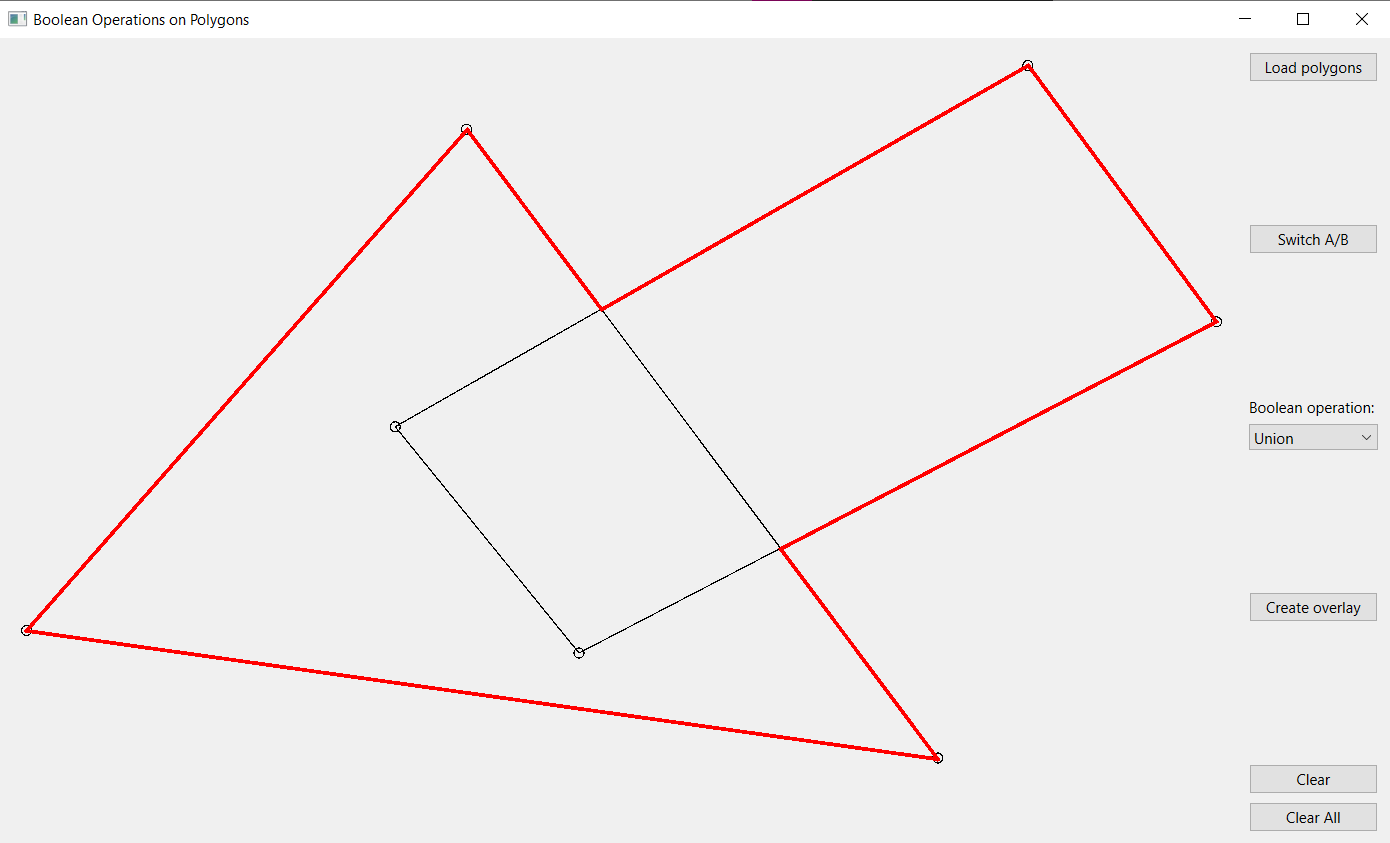
\includegraphics[scale=0.42]{images/vystup_union.png} 
	\caption{Sjednocení polygonů}
	\label{fig:vystup_union}
\end{figure} 
\begin{figure}[htbh]
	\centering
	\captionsetup{justification=centering}
	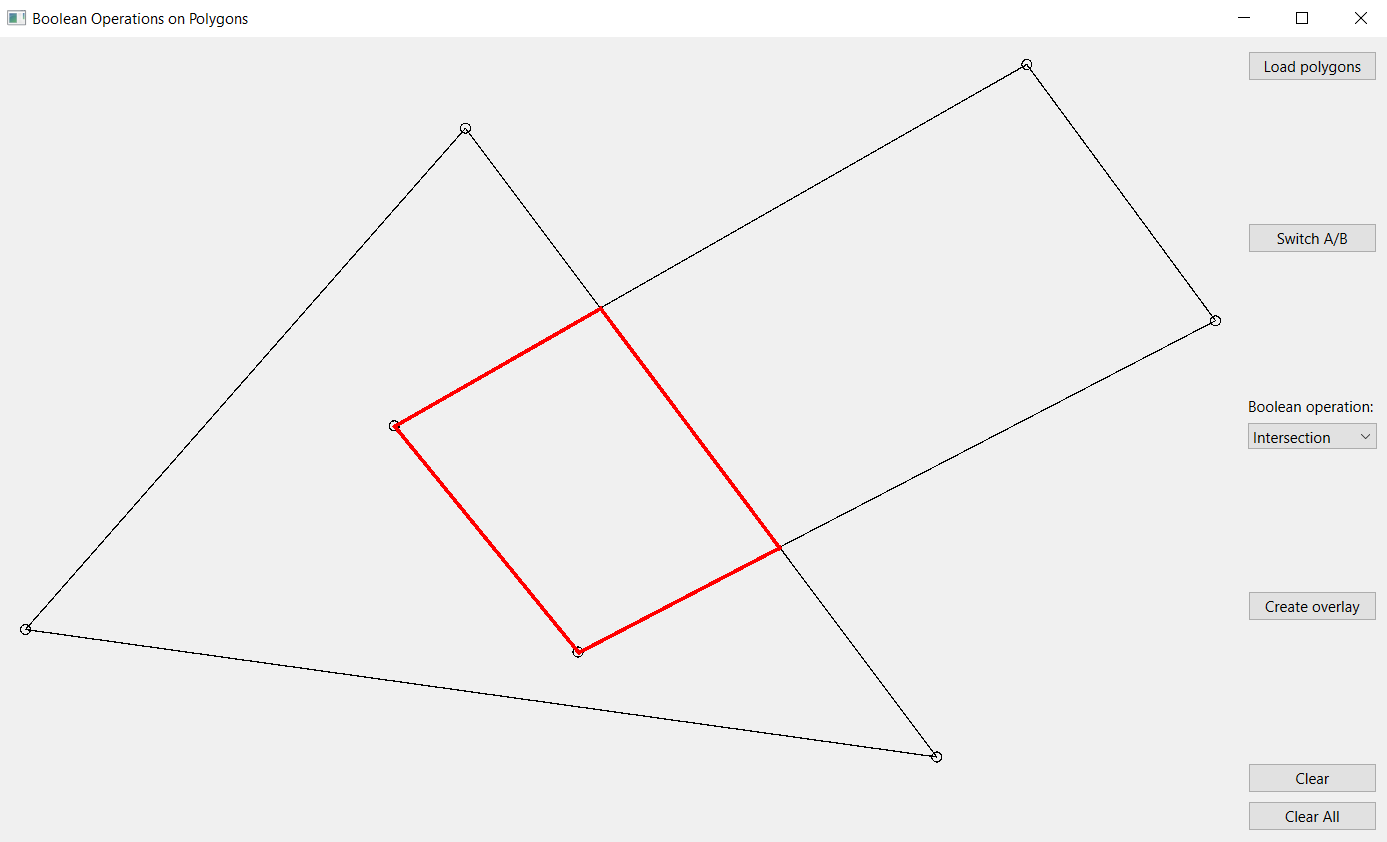
\includegraphics[scale=0.42]{images/vystup_intersection.png} 
	\caption{Průník polygonů}						\label{fig:vystup_intersection}
\end{figure} 
\begin{figure}[htbh]
	\centering
	\captionsetup{justification=centering}
	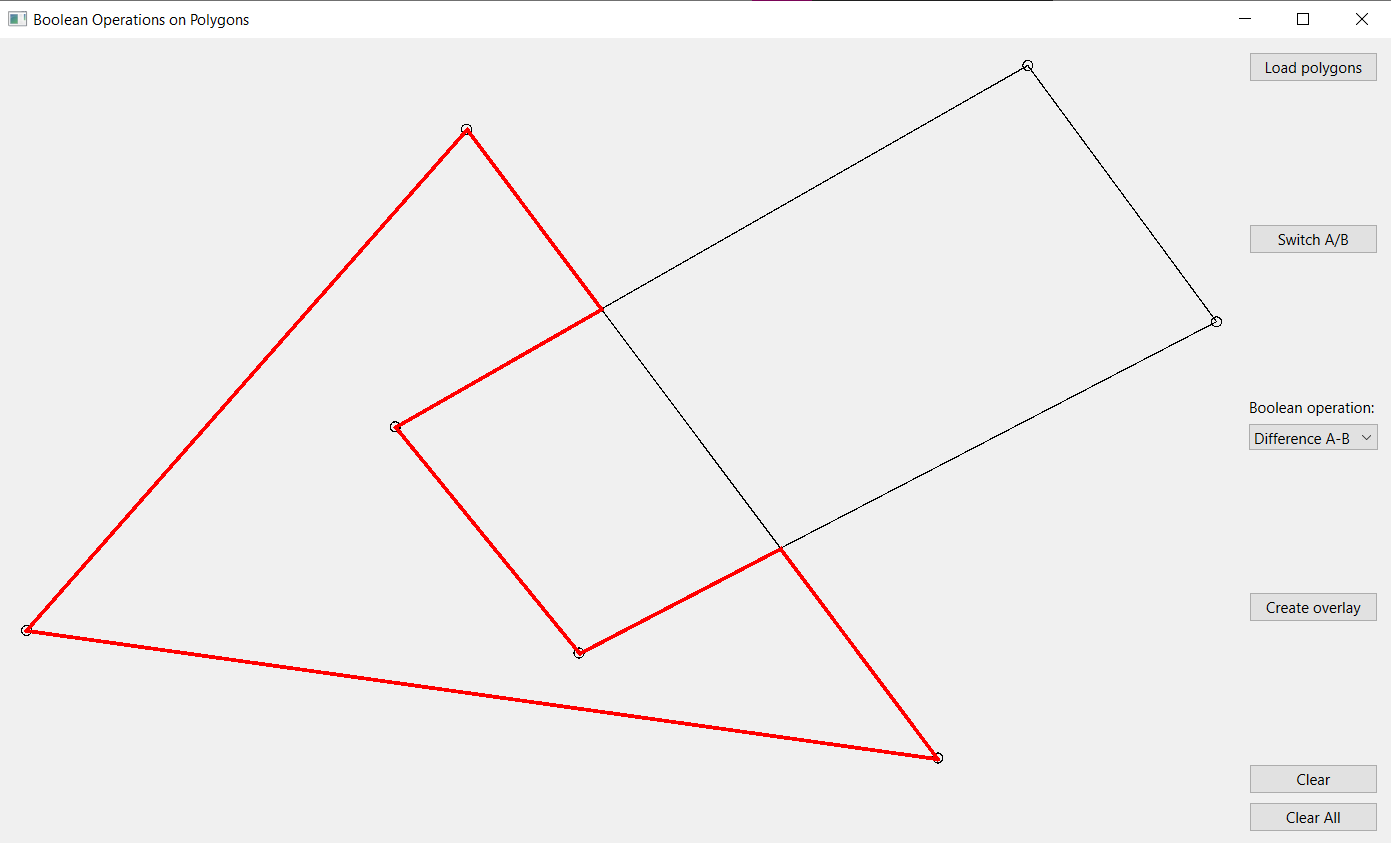
\includegraphics[scale=0.42]{images/vystup_diffAB.png} 
	\caption{Rozdíl polygonů A-B}	
	\label{fig:vystup_diffAB}
\end{figure} 
\begin{figure}[htbh]
	\centering
	\captionsetup{justification=centering}
	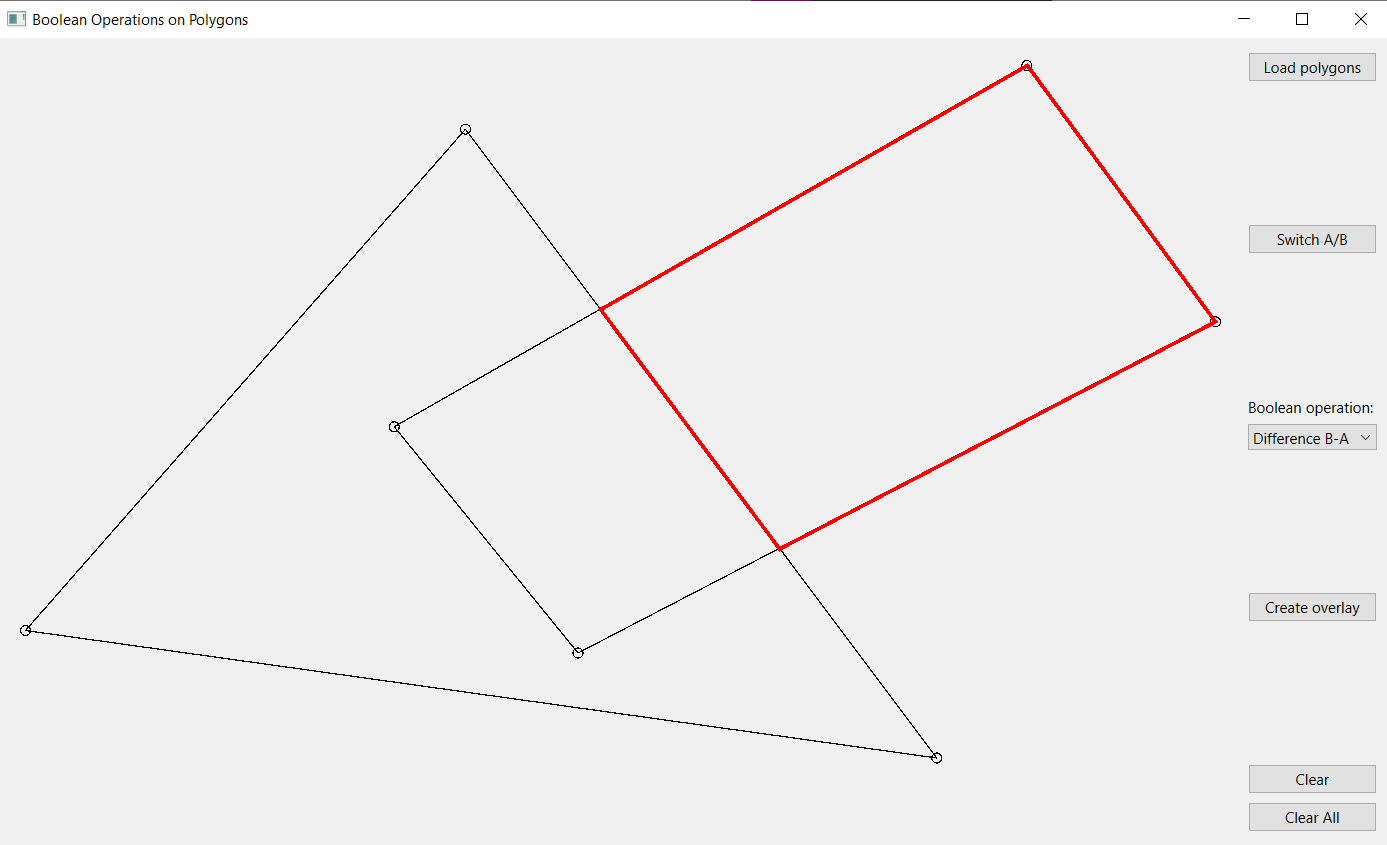
\includegraphics[scale=0.42]{images/vystup_diffBA.png} 
	\caption{Rozdíl polygonů B-A}	
	\label{fig:vystup_diffBA}
\end{figure} 
\clearpage

\section{Printscreen vytvořené aplikace}
\begin{figure}[htbh]
	\centering
	
	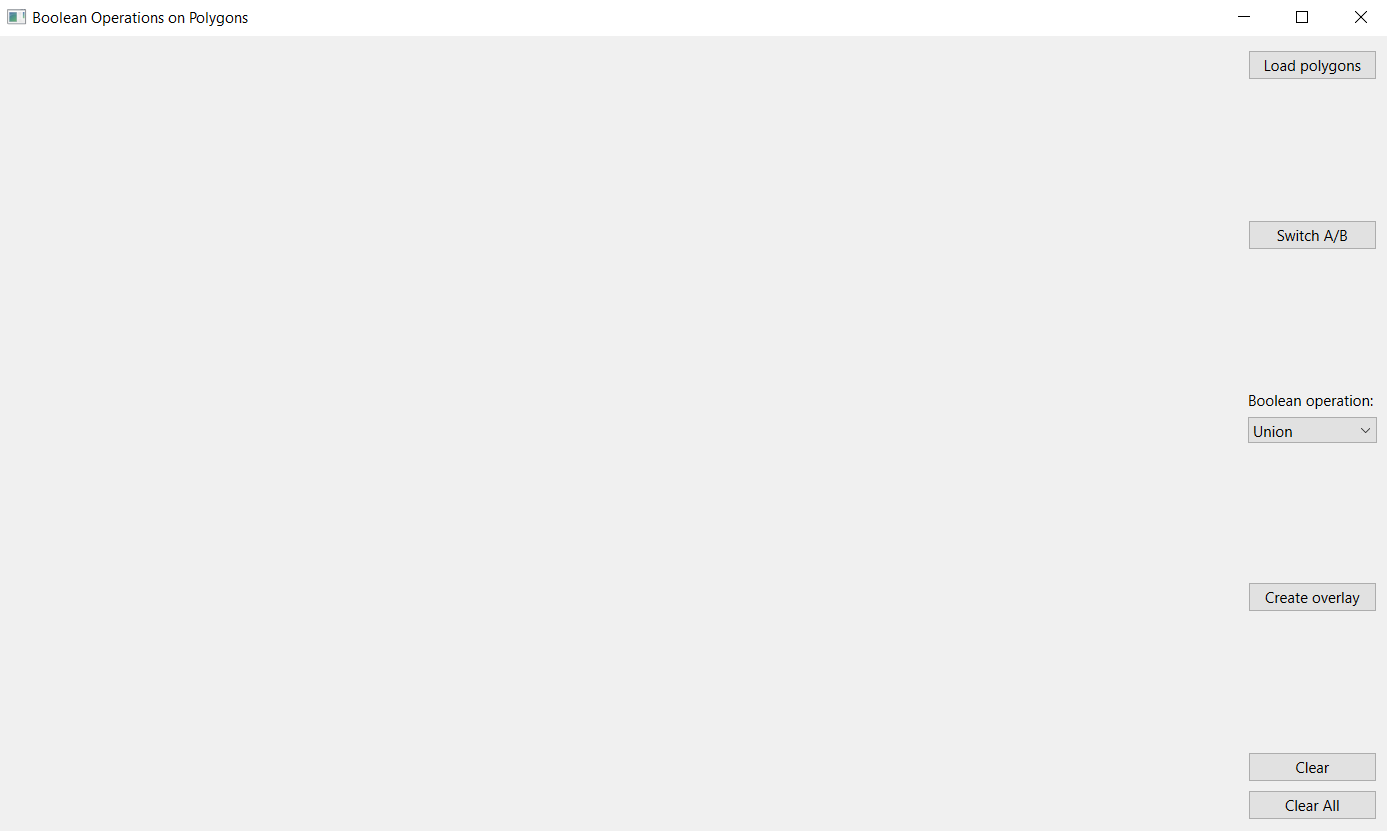
\includegraphics[scale=0.42]{images/aplikace_uvodni_okno.png} 
	\caption{Úvodní okno aplikace}
	\label{fig:uvodni_okno}
\end{figure} 
\FloatBarrier

\clearpage

%----------------------------------------------------------------------------------------
%	DOKUMENTACE
%----------------------------------------------------------------------------------------

\section{Dokumentace}
Kód zahrnuje celkem 7 tříd – Algorithms, Draw, Edge, QpointFBO, SortByX, SortByY Widget a jeden hlavičkový soubor Types. Všechny třídy budou následně detailněji popsány.   

\subsection{Hlavičkový soubor Types}
Hlavičkový soubor Types definuje následující výčtové typy.

\begin{itemize}
\item TPointLinePosition
\item TPointPolygonPosition
\item TBooleanOperation
\item T2LinesPosition
\item TPolygon
\item TEdges
\end{itemize}

\paragraph{TPointLinePosition}
TPointLinePosition ukládá hodnoty polohy bodu vůči přímce.

\begin{itemize}
\item RightHP v případě, že bod leží v pravé polorovině,
\item LeftHP v případě, že  bod leží v levé polorovině,
\item On v případě, že bod leží na přímce.
\end{itemize}

\paragraph{TPointPolygonPosition}
TPointPolygonPosition ukládá hodnoty polohy bodu vůči polygonu.

\begin{itemize}
\item Inner v případě, že bod uvnitř polygonu
\item Outer v případě, že  bod leží vně polygonu
\item Boundary v případě, že bod leží na hraně polygonu
\end{itemize}

\paragraph{TBooleanOperation}
TBooleanOperation definuje hodnoty pro určení typu množinové operace.

\begin{itemize}
\item Union - sjednocení polygonů
\item Intersection - průnik polygonů
\item DifferenceA\_B - rozdíl polygonů A-B
\item DifferenceB\_A - rozdíl polygonů B-A
\end{itemize}

\paragraph{T2LinesPosition}
TPointPolygonPosition ukládá hodnoty pro určení vzájemné polohy dvou přímek.

\begin{itemize}
\item Colinear - kolineární přímky
\item Parallel - rovnoběžné přímky
\item Intersect - různoběžné přímky
\item NonIntersect - mimoběžné přímky
\end{itemize}

\paragraph{TPolygon}
Představuje vektor datového typu QPointFBO.

\paragraph{TEdges}
Představuje vektor datového typu Edge

\subsection{Třída Algorithms}
Třída Algorithms obsahuje 9 funkcí:  

\begin{itemize}
	\item TPointLinePosition getPointLinePosition(QPointFBO \&a, QPointFBO \&p1, QPointFBO \&p2);
	\item double get2LinesAngle(QPointFBO \&p1, QPointFBO \&p2, QPointFBO \&p3, QPointFBO \&p4);
	\item TPointPolygonPosition getPositionWinding(QPointFBO \&q, TPolygon \&pol);
	\item std::tuple<QPointFBO,T2LinesPosition> get2LinesIntersection(QPointFBO \&p1, QPointFBO \&p2, QPointFBO \&p3, QPointFBO \&p4);
	\item void updatePolygons(TPolygon \&A, TPolygon \&B);
	\item void processIntersection(QPointFBO \&b, double t, int \&index, TPolygon \&P);
	\item void setEdgePositions(TPolygon \&A, TPolygon \&B);
	\item void selectEdges(TPolygon \&P, TPointPolygonPosition pos, TEdges \&edges);
	\item TEdges createOverlay(TPolygon \&A, TPolygon \&B, TBooleanOperation \&op);

\end{itemize}

\paragraph{TPointLinePosition getPointLinePosition(QPointFBO \&a, QPointFBO \&p1, QPointFBO \&p2);}
Analyzuje vzájemnou polohu mezi bodem a linií polygonu, resp. v jaké polorovině vůči linii se bod nachází. Vstupními argumenty funkce jsou souřadnice určovaného bodu (jako QPointFBO) a souřadnice 2 bodů určujících polohu linie (vrcholy polygonu taktéž jako QPointFBO). Funkce vrací vždy hodnotu RightHP, LeftHP, On datového typu TPointLinePosition dle následujících pravidel:

\begin{itemize}
\item RightHP v případě, že bod leží v pravé polorovině,
\item LeftHP v případě, že  bod leží v levé polorovině,
\item On v případě, že bod leží na linii.
\end{itemize}

\paragraph{double get2LinesAngle(QPointFBO \&p1, QPointFBO \&p2, QPointFBO \&p3, QPointFBO \&p4);}
Počítá úhel mezi dvěma liniemi. Vstupními argumenty jsou body určující linie, tzn. vrcholy polygonu. Návratovou hodnotou funkce je double – desetinné číslo s velikostí úhlu mezi těmito přímkami.  

\paragraph{TPointPolygonPosition getPositionWinding(QPointFBO \&q, TPolygon \&pol);}
Funkce analyzuje polohu boduvůči polygonu metodou Winding Number, jež byla podrobně vysvětlena v kapitole 3.  Vstupními argumenty je bod typu QPointFB a polygon datového typu TPolygon. Výstupní hodnotou je datový typ TPointPolygonPosition, jehož hodnoty nabývají následující hodnoty: 

\begin{itemize}
\item Inner v případě, že bod uvnitř polygonu
\item Outer v případě, že  bod leží vně polygonu
\item Boundary v případě, že bod leží na hraně polygonu
\end{itemize}

\paragraph{std::tuple<QPointFBO,T2LinesPosition> get2LinesIntersection(QPointFBO \&p1, QPointFBO \&p2, QPointFBO \&p3, QPointFBO \&p4);}
Funkce určuje vzájemnou polohu dvou přímek na základně hodnot parametrů k1, k2 a k3, které se vypočetly jako dílčí determinanty směrových vektorů u,v,w.
Pokud se všechny parametry k blíží k nule, vrací funkce dvojici hodnot QPointFBO s defaultními parametry a hodnotu \textbf{Colinear} datového typu T2LinesPosition. Pokud se blíží nule pouze koeficienty k1 a k2, vrací funkce QPointFBO s defaultními parametry a \textbf{Parallel}. Dále se vypočtou hodnoty $\alpha$ a $\beta$. Pokud se hodnoty nacházejí v intervalu (0,1), vypočte se pozice průsečíku. Následně funkce vrací hodnotu \textbf{Intersect} a bod QPointFBO s vypočtenými sořadnicemi a parametry $\alpha$ a $\beta$. Pokud nenastane ani jedna z výše popsaných situací, vrací funkce bod QPointFBO a hodnotu \textbf{NonIntersect} dat. typu T2LinesPosition.

\paragraph{void updatePolygons(TPolygon \&A, TPolygon \&B);}
Funkce hledá průsečíky dvou polygonů pomocí funkce \textit{get2LinesIntersection()}. Pokud průsečík existuje, uloží se do mapy, jejíž klíčem je parametr $\alpha$ nebo $\beta$ a hodnotou je vypočtený průsečík. Následně se bod přidá do daného polygonu pomocí funkce \textit{processIntersection}. Funkce nic nevrací.

\paragraph{void processIntersection(QPointFBO \&b, double t, int \&index, TPolygon \&P);}
Funkce je volána funkcí \textit{updatePolygons()}. Tato funkce vkládá nalezený průsečík s hodnotami $\alpha$ nebo $\beta$ na určitou pozici danou indexem v daném polygonu. Funkce nic nevrací.

\paragraph{void setEdgePositions(TPolygon \&A, TPolygon \&B);}
Funkce určuje pozici středových bodů všech hran polygonu vůči druhému polygonu. K určení vzájemné polohy body a polygonu se volá funkce \textit{getPositionWinding()}. Settrem se každému vrcholu polygonu nastaví hodnota TPointPolygonPosition. Funkce nic nevrací.

\paragraph{void selectEdges(TPolygon \&P, TPointPolygonPosition pos, TEdges \&edges);}
Funkce přidává do vektoru hran TEdges ty hrany polygonu P, jejichž počáteční body mají hodnotu TPointPolygonPosition shodnou se vstupní hodnotou pos. Funkce nic nevrací.

\paragraph{TEdges createOverlay(TPolygon \&A, TPolygon \&B, TBooleanOperation \&op);}
Funkce vrací ty hrany obou polygonů, které odpovídají vstupní hodnotě TBooleanOperation, která odpovídá zvolené množinové operaci. Funkce nejdříve vypočte průsečíky polygonů a aktualizuje je pomocí funkce \textit{updatePolygons()}. Následně se určí vzájemnou polohu hran vůči oboum polygonům pomocí funkce \textit{setEdgePositions()}. Následně se opakovaně volá funkce selectEdges na základně vybrané množinové operace. Pokud je zvolena operace \textbf{Union} (sjednocení), vyberou se vnější hrany obou polygonů. Pokud se zvolí operace \textbf{Intersection} (průnik), za výsledek se uvažují pouze vnitřní hrany obou polygonů. Pokud je vybrána operace \textbf{Difference A-B}, vrátí funkce vnější hrany polygonu A a vnitřní hrany polygonu B. Pokud zvolíme operaci \textbf{Difference B-A}, vyberou se naopak vnitřní hrany hrany polygonu A a vnější hrany polygonu B.

\subsection{Třída Draw}
Třída Draw obsahuje následující funkce, které budou dále podrobně popsány:

\begin{itemize}
\item void paintEvent(QPaintEvent *event);
\item void mousePressEvent(QMouseEvent *event);
\item void switchSource(){addA = !addA;}
\item void drawPolygon(TPolygon \&pol, QPainter \&qp);
\item TPolygon getA(){return A;}
\item TPolygon getB(){return B;}
\item void setEdges(TEdges \&edg){res = edg;}
\item void clear(){res.clear();}
\item void clearAll(){A.clear(); B.clear(); res.clear();}
\item void loadData(QString \&file\_name);
\end{itemize}

a následující proměnné:

\begin{itemize}

\item TPolygon A, B;
\item TEdges res;
\item bool addA;
\item double y\_max = 0, x\_min = 999999999; //pro transformaci
\item double y\_min = 999999999, x\_max = 0; //pro meritko
\end{itemize}

\paragraph{void paintEvent(QPaintEvent *event);}
Funkce nastavuje grafické atributy vykreslovaných objektů a kreslí na plátno zadané polygony a znázorňuje výsledky množinových operací.

\paragraph{void mousePressEvent(QMouseEvent *event);}
Metoda získává souřadnice kursoru myši, ukládá je do polygonu a následně je vykresluje na plátno.

\paragraph{void switchSource();}
Metoda je volána po kliknutí na tlačítka \textbf{Switch A/B} a přepíná aktivní polygon.

\paragraph{void drawPolygon(TPolygon \&pol, QPainter \&qp);}
Metoda transformuje polygon na Qpolygon a vykresluje ho na plátno.

\paragraph{TPolygon getA();}
Funkce pro vrácení polygonu A ze třídy Draw.

\paragraph{TPolygon getB();}
Funkce pro vrácení polygonu A ze třídy Draw.

\paragraph{void setEdges(TEdges \&edg){res = edg;}}
Metoda ukládá vybrané hrany zadanou množinovou operací ze třídy Widget do třídy Draw.

\paragraph{void clear();}
Metoda slouží pro odstranění výsledku množinové operace.

\paragraph{void clearAll();}
Funkce odstraňuje obsah vykreslovacího plátna.

\paragraph{void loadData(QString \&file\_name);}
Funkce načítá data z textového souboru a ukládá je do polygonů A a B. Vstupní argumentem je cesta k souboru, jejž chceme načíst do aplikace. 

\subsection{Třída Edge}
Ve třídě Edge je definován datový typ Edge, jenž definuje hranu polygonu. Hrana je definována počátečním a koncovým bodem uloženými v datovém typu QPointFBO. Funkce je opatřena gettry a settry.

\subsection{Třída QPointFBO}
Třída definuje datový typ QPointFBO, jež je dědičným datovým typem QPointF. Třída obsahuje soukromé proměnné alfa beta a pos, která ukládá pozici bodu vůči polygonu. Funkce je opatřena sadou gettrů a settrů.

\subsection{Třída SortByX}
Třída definuje operátor přetížení, který řadí body podle x-ové souřadnice.

\subsection{Třída SortByY}
Třída definuje operátor přetížení, který řadí body podle y-ové souřadnice.

\subsection{Třída Widget}
Třída Widget obsahuje 13 metod:

\begin{itemize}
\item void on\_pushButton\_clicked();
\item void on\_pushButton\_2\_clicked();
\item void on\_pushButton\_3\_clicked();
\item void on\_pushButton\_4\_clicked();
\item void on\_pushButton\_5\_clicked();
\end{itemize}

\paragraph{on\_pushButton\_clicked();}
Funkce po stisknutí tlačítka \textbf{Switch A/B} volá funkci \textit{switchSource()} ze třídy \textit{Draw}

\paragraph{on\_pushButton\_2\_clicked();}
Funkce po stisknutí tlačítka \textbf{Create overlay} volá na základě zvolené množinové operace v \textit{comboBoxu} metodu \textit{createOverlay()} ze třídy \textit{Algorithms} a vyhovující hrany ukládá setterem do třídy \textit{Draw}.

\paragraph{on\_pushButton\_3\_clicked();}
Funkce po stisknutí tlačítka \textbf{Clear} volá metodu \textit{clear()} ze třídy \textit{Draw}. 

\paragraph{on\_pushButton\_4\_clicked();}
Funkce po stisknutí tlačítka \textbf{Clear All} volá metodu \textit{clearAll()} ze třídy \textit{Draw}. 

\paragraph{on\_pushButton\_5\_clicked();}
Funkce po stisknutí tlačítka \textbf{Load polygons} volá metodu \textit{loadData()} ze třídy \textit{Draw} a tím načítá soubor vybraný přes dialogové okno.

%----------------------------------------------------------------------------------------
%	ZÁVĚR
%----------------------------------------------------------------------------------------

\section{Závěr}
V rámci úlohy byla vytvořena aplikace s grafickým rozhraním, která umožňuje provádět základní množinové operace nad dvěma polygony. Polygony lze do aplikace načíst dvěma způsoby. První možnost zahrnuje načítání z textového souboru. Aby bylo zajištěno správné načítání, musí soubor splňovat specifický datový formát. Alternativou je zadávat polygony manuálně. V tomto případě musí uživatel naklikat kursorem myší alespoň tři body u prvního polygonu a tlačítkem \textit{Switch A/B} se přepnout do druhého polygonu a opět definovat jeho tvar. Abychom však mohli operace provádět, musí být zajištěno, že se oba polygony překrývají. Po načtení souboru pak lze provádět překryvné operace typu sjednocení, průnik a rozdíly polygonu A-B či B-A. Výsledek se v aplikaci zobrazí zvýrazněním hran tlustou červenou barvou. Výsledek operací lze pak příslušným tlačítkem odstranit, případně lze vyčistit celé plátno.

\end{document}
